% Options for packages loaded elsewhere
\PassOptionsToPackage{unicode}{hyperref}
\PassOptionsToPackage{hyphens}{url}
\documentclass[
]{article}
\usepackage{xcolor}
\usepackage[margin=1in]{geometry}
\usepackage{amsmath,amssymb}
\setcounter{secnumdepth}{-\maxdimen} % remove section numbering
\usepackage{iftex}
\ifPDFTeX
  \usepackage[T1]{fontenc}
  \usepackage[utf8]{inputenc}
  \usepackage{textcomp} % provide euro and other symbols
\else % if luatex or xetex
  \usepackage{unicode-math} % this also loads fontspec
  \defaultfontfeatures{Scale=MatchLowercase}
  \defaultfontfeatures[\rmfamily]{Ligatures=TeX,Scale=1}
\fi
\usepackage{lmodern}
\ifPDFTeX\else
  % xetex/luatex font selection
\fi
% Use upquote if available, for straight quotes in verbatim environments
\IfFileExists{upquote.sty}{\usepackage{upquote}}{}
\IfFileExists{microtype.sty}{% use microtype if available
  \usepackage[]{microtype}
  \UseMicrotypeSet[protrusion]{basicmath} % disable protrusion for tt fonts
}{}
\makeatletter
\@ifundefined{KOMAClassName}{% if non-KOMA class
  \IfFileExists{parskip.sty}{%
    \usepackage{parskip}
  }{% else
    \setlength{\parindent}{0pt}
    \setlength{\parskip}{6pt plus 2pt minus 1pt}}
}{% if KOMA class
  \KOMAoptions{parskip=half}}
\makeatother
\usepackage{graphicx}
\makeatletter
\newsavebox\pandoc@box
\newcommand*\pandocbounded[1]{% scales image to fit in text height/width
  \sbox\pandoc@box{#1}%
  \Gscale@div\@tempa{\textheight}{\dimexpr\ht\pandoc@box+\dp\pandoc@box\relax}%
  \Gscale@div\@tempb{\linewidth}{\wd\pandoc@box}%
  \ifdim\@tempb\p@<\@tempa\p@\let\@tempa\@tempb\fi% select the smaller of both
  \ifdim\@tempa\p@<\p@\scalebox{\@tempa}{\usebox\pandoc@box}%
  \else\usebox{\pandoc@box}%
  \fi%
}
% Set default figure placement to htbp
\def\fps@figure{htbp}
\makeatother
\setlength{\emergencystretch}{3em} % prevent overfull lines
\providecommand{\tightlist}{%
  \setlength{\itemsep}{0pt}\setlength{\parskip}{0pt}}
\usepackage{helvet}
\renewcommand*\familydefault{\sfdefault}
\usepackage{setspace}
\doublespacing
\usepackage[left]{lineno}
\usepackage{bookmark}
\IfFileExists{xurl.sty}{\usepackage{xurl}}{} % add URL line breaks if available
\urlstyle{same}
\hypersetup{
  hidelinks,
  pdfcreator={LaTeX via pandoc}}

\author{}
\date{\vspace{-2.5em}}

\begin{document}

\section{Resolving gut microbiome networks within
Chiropterans}\label{resolving-gut-microbiome-networks-within-chiropterans}

Timothy J. Rogers, Laurel R. Yohe, Richard A. White \({\dagger}\)

Department of Bioinformatics, University of North Carolina, Charlotte,
NC 28223; Department of Bioinformatics and Genomics, North Carolina
Research Center (NCRC), Kannapolis, NC

\({\dagger}\) To whom correspondence should be addressed

\newpage

\subsection{Abstract (250 words)}\label{abstract-250-words}

\newpage

\subsection{Introduction}\label{introduction}

\begin{itemize}
\tightlist
\item
  Bats are known carriers of human associated pathogens
\item
  The reason bats are bioreactors is not understood
\item
  The diet of bats may contribute to the gut microbiota makeup
\item
  Phage associated with these microbiota can benifit and hinder
  microbial populations and have an impack on bat immune responses
\item
  Some ideas suggest viral tolerance is linked to

  \begin{itemize}
  \tightlist
  \item
    Uniqueness of bats and their variation in Diets

    \begin{itemize}
    \tightlist
    \item
      Diversity
    \item
      Ecological role
    \item
      Pathogenic role
    \end{itemize}
  \end{itemize}
\item
  Methods for characterizing microbiome and virome. As well as methods
  for linking the two

  \begin{itemize}
  \tightlist
  \item
    Culture dependant vs independent

    \begin{itemize}
    \tightlist
    \item
      What has been discovered with these methods
    \item
      How these methods have been applied to bats

      \begin{itemize}
      \tightlist
      \item
        What has been found
      \item
        What has yet to be discribed
      \end{itemize}
    \end{itemize}
  \end{itemize}
\item
  Goal of this study
\end{itemize}

\subsection{Materials and Methods}\label{materials-and-methods}

\begin{itemize}
\tightlist
\item
  Sample location discription
\item
  Sample collection
\item
  Sample processing \#\#\# Phase genomics portion
\item
  (AND)
\end{itemize}

\subsubsection{In house analysis of MAGs, vcontigs, and viral-host
pairing}\label{in-house-analysis-of-mags-vcontigs-and-viral-host-pairing}

\paragraph{vOTU curration}\label{votu-curration}

\begin{itemize}
\tightlist
\item
  (AND) Genomad (v x.x.x) was used to varify contigs identified as viral
  by phase genomics and for taxonomic identification.
\item
  (AND) We also ran all assembly files from phase genome through genomad
  to identify potential viral sequences that the phase genome pipeline
  may have missed
\item
  (AND) Quality filtered viral sequences were then clustered into
  species-level equivalent viral operational taxanomic units (vOTUs) at
  95\% average nucleatide identity over 85\% of the alignment fraction
  of the shorter sequence using the greedy centroid algorithm
  (anicalc.py and aniclust.py) from checkV (v x.x.x).
\end{itemize}

\paragraph{MAG curration}\label{mag-curration}

\begin{itemize}
\tightlist
\item
  (AND) MAGs from phase metagenomic were quality filtered using checkM
  (v x.x.x).
\item
  (AND) Quality filtered MAGs were then dereplicated using dRep (v
  x.x.x) at 99\% ANI with the following settings (--S\_algorithm
  fastANI, -comp 50, --SkipMash)
\item
  (AND) MAGs representatives were taxonomically identified using the
  Genome Taxonomy Database Toolkit (GTDB-Tk v x.x.x)
\end{itemize}

\paragraph{vOTU and MAG coverage}\label{votu-and-mag-coverage}

\begin{itemize}
\tightlist
\item
  (AND) Quality controled reads were mapped to the vOTUs and
  representative MAGs using bowtie (v x.x.x) and sam files were
  converted to indexed and sorted bam files using samtools (v x.x.x).
\item
  (AND) Bam files were then fed into anvi'o (v x.x.x) to calculate the
  Q2Q3 coverage of vOTUs and MAGs across bat species.
\item
  (AND) Q2Q3 coverages for both vOTUs and MAGs were then normalized by
  sequence length.
\item
  (AND) For alpha diveristy analyzes, normalized Q2Q3 coverages for both
  vOTUs and MAGs were rarefied using the rrarify function of the vengan
  R package.
\item
  (AND) For beta diversity analyzes, normalized Q2Q3 coverages for both
  vOTUs and MAGs were used to create rarefied Hellinger distance
  matrices using the vegan (v x.x.x) and labdsv (v x.x.x) R packages.
\item
  (AND) For abundance pattern analyzes, normalized Q2Q3 coverages were
  coverted into units of GCPM (Genome Copy Per Million Reads) for MAGs,
  as laid out in Rogers et al.~2022 (citation), and TPM (Transcripts Per
  Million Reads) for vOTUs.
\item
  (AND) Abundance correlations of vOTUs and MAGs across and within
  samples were determined using hierarchical clustering of Spearman rank
  correlation distance matrice in base R (v x.x.x).
\end{itemize}

\paragraph{Metabolic predictions}\label{metabolic-predictions}

\begin{itemize}
\tightlist
\item
  The program metacerberus (v x.x.x) was used for gene anotation of both
  viral sequences and MAGs using the following data bases: Functional
  Ontology Assignments for Metagenomes (FOAM), KEGG, CAZy/dbCAN, VOG,
  pVOG, PHROG, and COG.
\end{itemize}

\paragraph{AMR and CAZY gene abundance
patterns}\label{amr-and-cazy-gene-abundance-patterns}

\begin{itemize}
\tightlist
\item
  (AND) Read coverage and abundance for AMR and CAZY genes were
  calculated using a custom ihhouse script.
\end{itemize}

\paragraph{Linking virus to host}\label{linking-virus-to-host}

\begin{itemize}
\tightlist
\item
  (AND) IPHoP (v x.x.x) was used to link all viral sequences to all
  medium to high quality MAGs, not just to the representative vOTUs and
  MAGs.
\item
  (AND) The viral and MAG IDs of those within the viral-host predictions
  from both IPHoP and Phase genomes were replaced with the corresponding
  representative vOTU and MAG IDs.
\end{itemize}

\paragraph{Statistical analysis}\label{statistical-analysis}

\begin{itemize}
\tightlist
\item
  (AND) Differences in MAG and vOTU composition among bat species were
  analyzed via distance based redundancy analysis (db-RDA) on a
  quntitative Hellinger distance matirx.
\item
  (AND) The richness and evenness of MAGs and vOTUs were compared using
  the R package microbiome for richness (chao1) and the package hillR (v
  x.x.x) for evenness (Pielou's index).
\item
  (AND) Statistical significants was determined based on 9999
  permutations of the data in the vegan R package.
\end{itemize}

\subsection{Results}\label{results}

\subsubsection{MAGs}\label{mags}

\begin{itemize}
\item
  (AND) We recovered 5 Archaeal and 182 Bacterial medium to high quality
  MAGs with \(\geq\) 50 \% and \(\leq\) 9 \% redundancy.
\item
  (AND) Of these 187 MAGs, 106 were \(\geq\) 90\% complete and \(\leq\)
  10\% redundant, while YY are of high quality as determined by
  parameters layed out in XXX et al.~(** TABLE **).
\item
  (AND) \emph{Bacillota}, \emph{Actinomycetota}, and
  \emph{Pseudomonadata} were the predominate phylum across the gut
  microbiome within all 3 of the bat species (\textbf{Figure}).
\item
  (AND) No significant differnces were found in the richness (Choa1) or
  evenness (Pielou's Index) of prokaryotic MAGs across the 3 bat
  species.
\item
  (AND) db-RDA analysis revealed no significant differnce in the
  \(B\)-diversity of the prokaryotic MAGs across the 3 bat species.
\end{itemize}

\begin{figure}
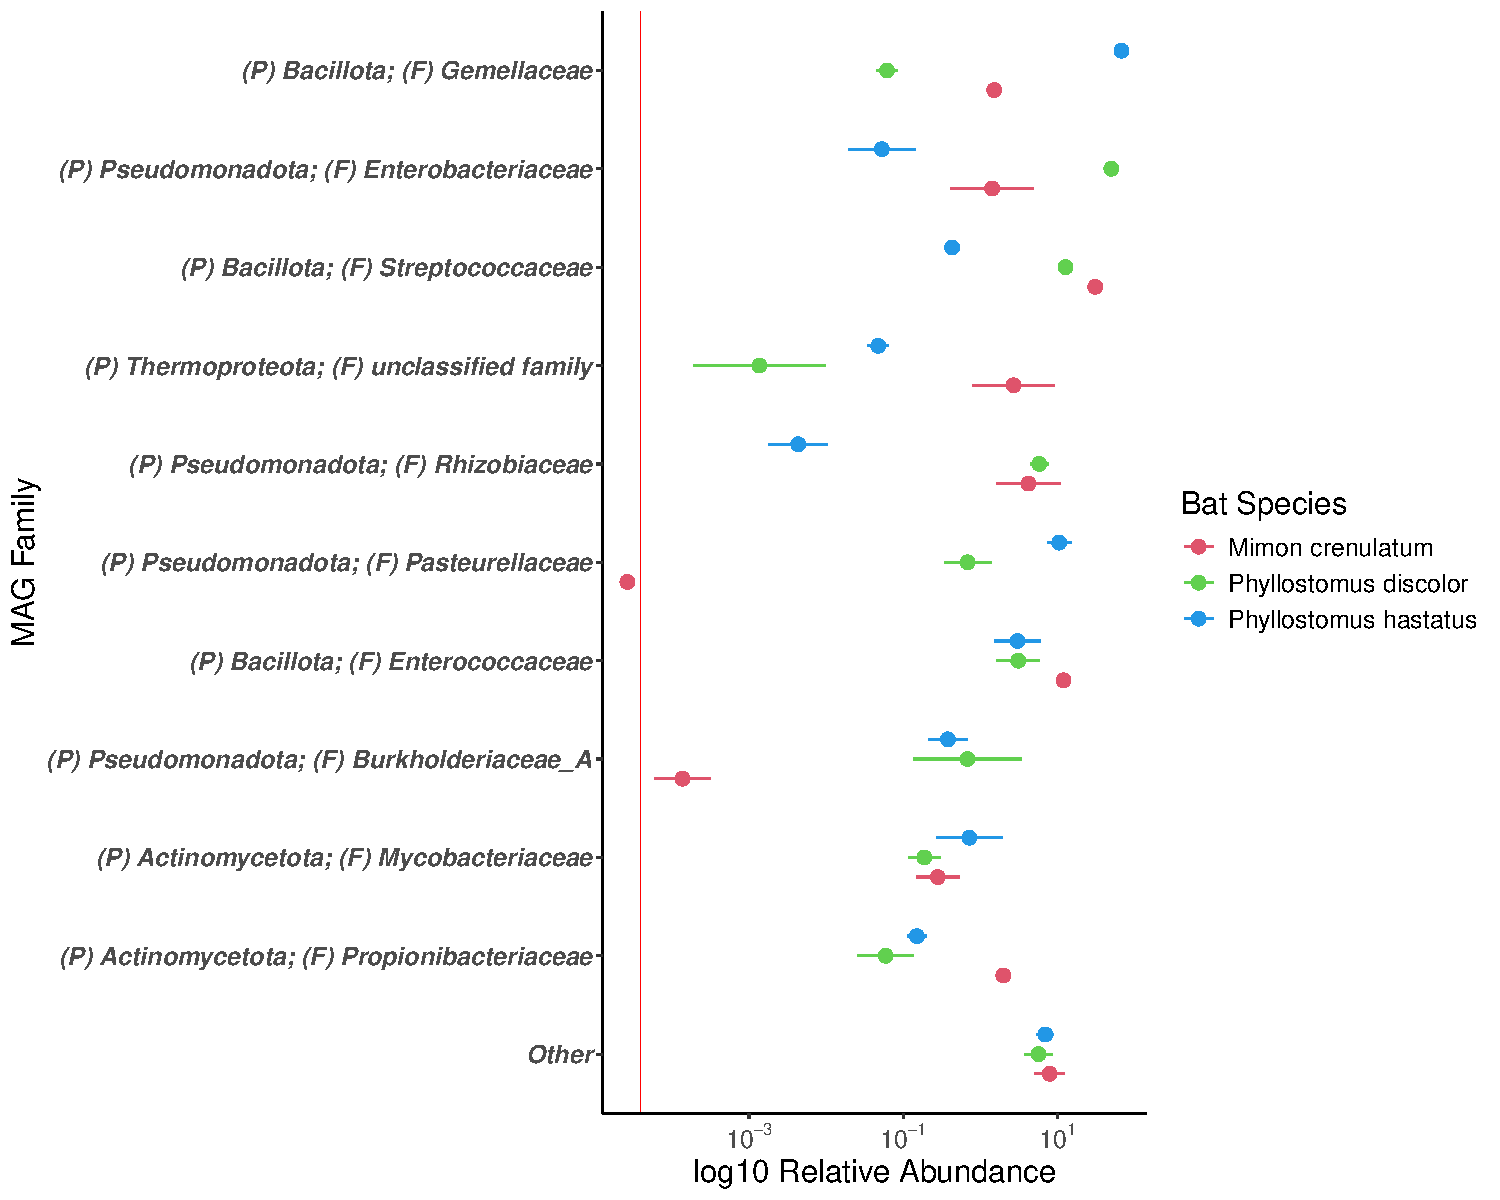
\includegraphics[width=400px,height=350px]{../../data/results/figures/FigX_top10_most_abun_mag_taxa} \caption{Distribution of the top 10 most abundant prokaryotic families across the gut microbiome of the three bat species}\label{fig:FigX}
\end{figure}

\subsubsection{vOTUs}\label{votus}

\begin{itemize}
\tightlist
\item
  (AND) A total of 17702 potential viral sequences were ID from the 6
  individual assemblies.
\item
  (AND) Clustering at 95\% ANI over 85\% of the shortest sequence
  identified 16289 viral operational taxanomic units (vOTUs) that were
  \(\geq\) 1 kbp in length.
\item
  (AND) Further filtering for sequences \(\geq\) 2.5 kpb resulted in a
  final set of 6235 vOTUs.
\item
  (AND) After rarefaction, 5582 vOTUs were retained.
\item
  (AND) CheckV was used to assess the quality of these sequences,
  revealing that 361 (6\%) were \(\geq\) 50\% complete including 39
  complete vOTUs that identified on the bases of direct terminal repeats
  (DTR), 74 high quality vOTUs that were identified on the bases of AAI
  (54 vOTUs) and HMM (20 vOTUs), 198 medium quality vOTUs that were
  idenified on the bases on AAI (136 vOTUs) and HMM (62 vOTUs), and 50
  low quality vOTUs that were identified based on AAI (41 vOTUs) and HMM
  (9 vOTUs). The reset of the vOTUs (5221) were of low quality (3298) or
  the quality was undetermined (1923).
\item
  (AND) An unclassified order of the class \emph{Caudoviricetes},
  families \emph{Retroviridae}, \emph{Adintoviridae}, and
  \emph{Iridoviridae}, an unclassified family of \emph{Kyanoviridae},
  families \emph{Inoviridae} and \emph{Bornaviridae}, an unclassified
  family of \emph{Herelleviridae}, families \emph{Mimiviridae} and
  \emph{Parvoviridae} were the most predominate viral taxa across the
  gut virome with all 3 of the bat species (\textbf{Figure}).
\item
  (But) No statistically significant differences were found in the viral
  richness, envenness, or \(B\)-diversity nor did indicator analysis
  reveal any indicator viral spices for the bat species.
\end{itemize}

\begin{figure}
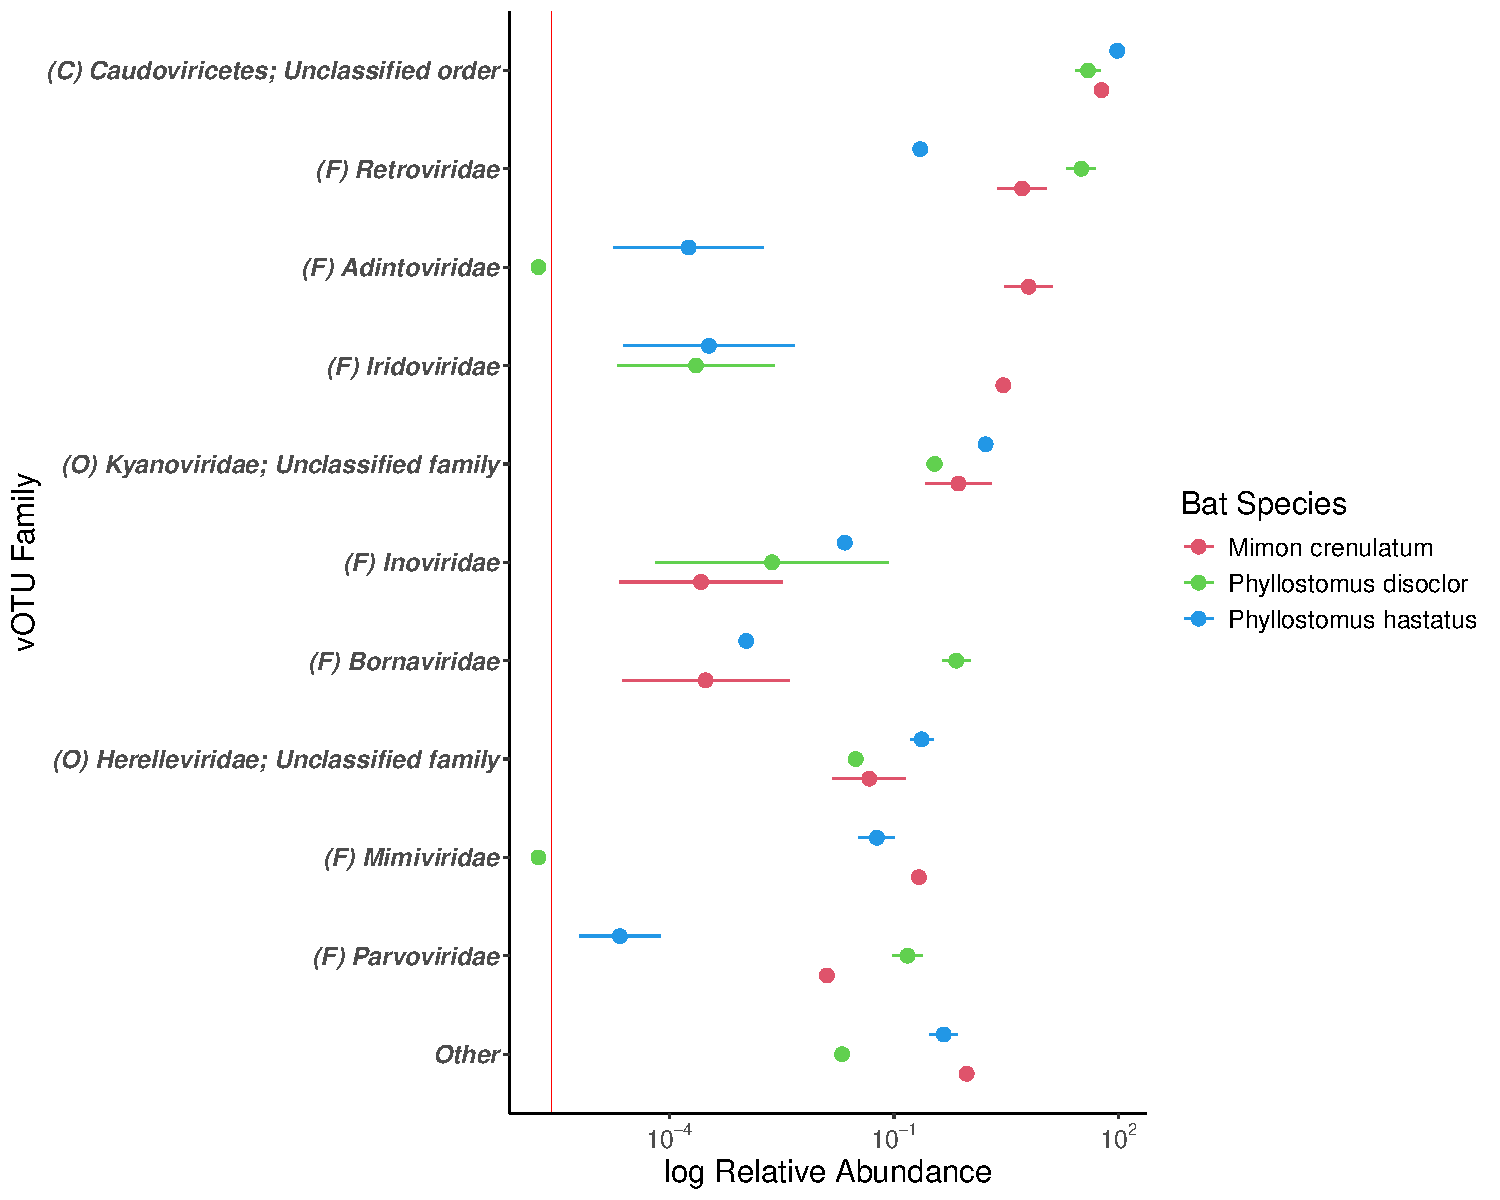
\includegraphics[width=400px,height=350px]{../../data/results/figures/FigX_top10_most_abun_viral_taxa} \caption{Distribution of the top 10 most abundant viral families across the gut virome of the three bat species}\label{fig:FigY}
\end{figure}

\paragraph{Metabolic capabilities}\label{metabolic-capabilities}

\begin{itemize}
\tightlist
\item
  (AND)
\end{itemize}

\subsubsection{Virus-host predicitons}\label{virus-host-predicitons}

\begin{itemize}
\tightlist
\item
  (AND) A total of 1308 viru-host prodictions were made using phase HiC
  and IPHoP methods.
\item
  (AND) These predictions included 186 MAGs and 953 vOTUs.
\item
  (AND) Of these, 352 were made by only phase, 867 were made by only
  IPHoP, and 80 were agreed matches between both methods
  (\textbf{Figure}).
\item
  (AND) Of those predictions made by IPHoP, 565 are based on blastn and
  391 are based on iPHoP-RF
\item
  (AND) MAGs within the bacteria phyla \emph{Actinomycetota},
  \emph{Bacillota}, \emph{Pseudomonadota}, and \emph{Desulfobacterota}
  had the highest frequency of being targeted by viruses (84, 62, 18,
  and 13 MAGs respectively).
\item
  (AND) Host families most often targeted within \emph{Actinomycetota}
  include \emph{Mycobacteriaceae} (20 MAGs) and \emph{Nocardiaceae} (10
  MAGs).
\item
  (AND) The host family most often targeted within \emph{Bacillota} is
  \emph{Enterococcaceae} (15 MAGs).
\item
  (AND) The host family most often targeted within \emph{Pseudomonadota}
  is \emph{Enterobacteriaceae} (6 MAGs).
\item
  (AND) The host family most often targeted within
  \emph{Desulfovibrionaceae} is \emph{Desulfobacterota} (9 MAGs).
\end{itemize}

\begin{figure}
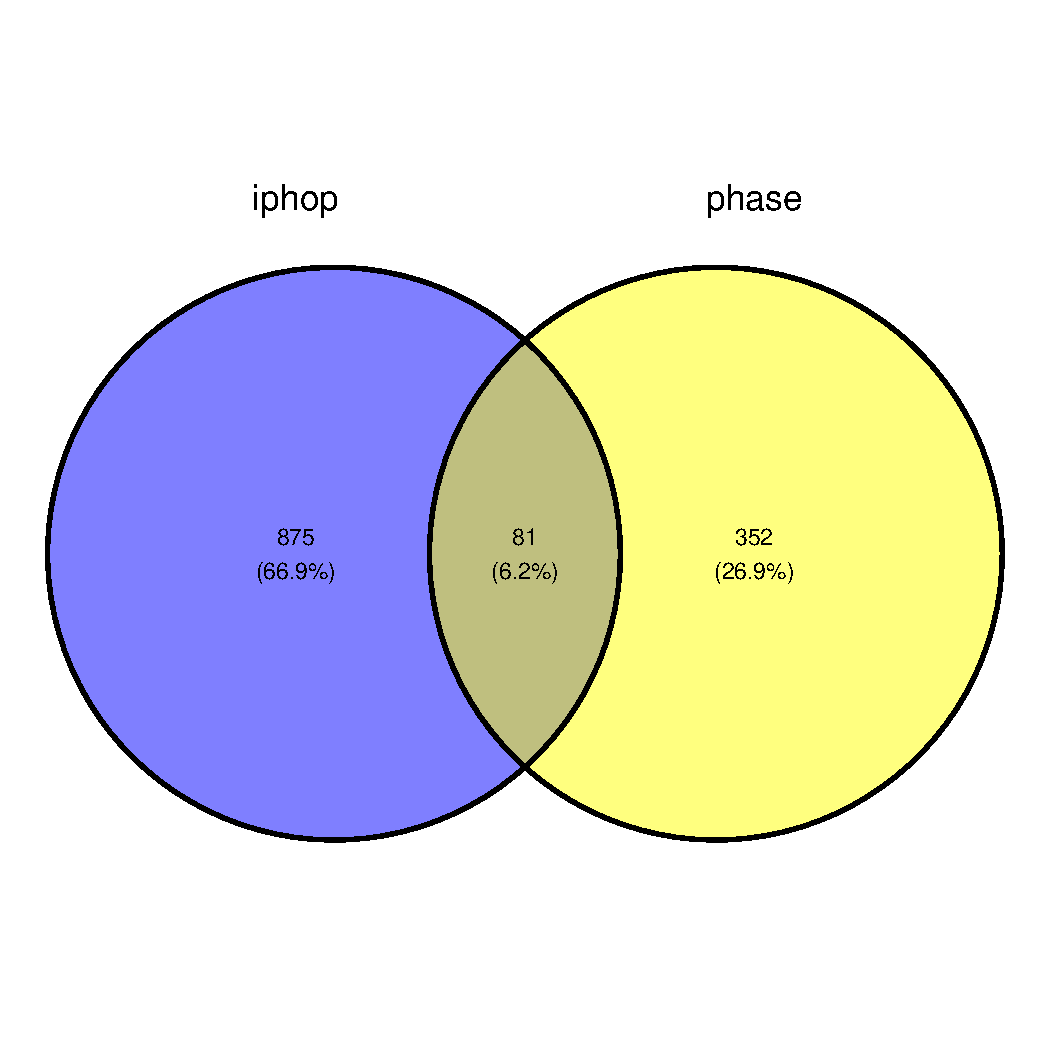
\includegraphics[width=400px,height=350px]{../../data/results/figures/updated_venndiagram_phase_iphop} \caption{Venn diagram showing the number of virus-host predictions made by each method used}\label{fig:FigZ}
\end{figure}

\begin{figure}
\includegraphics[width=400px,height=350px]{../../data/results/figures/Bat_gut_viral_host_network_figure} \caption{Virus-host network analysis}\label{fig:FigA}
\end{figure}

\subsection{Descusion}\label{descusion}

\begin{itemize}
\tightlist
\item
  (AND) The families \emph{Mycobacteriaceae} and \emph{Nocardiaceae}
  within the bacteria phylum \emph{Actinomycetota} contain known
  pathogenic members (\textbf{CITATION}).
\item
  (AND) The family \emph{Enterococcaceae} within the bacteria phylum
  \emph{Bacillota} contains known pathogenic members
  (\textbf{CITATION}).
\item
  (AND) The family \emph{Enterobacteriaceae} within the bacteria phylum
  \emph{Pseudomonadota} contain known pathogenic memebers
  (\textbf{CITATION}).
\item
  (AND) The family \emph{Desulfovibrionaceae} within the bacteria phylum
  \emph{Desulfobacterota} contain known opportunistic pathogenic members
  (\textbf{CITATION}).
\end{itemize}

Macro Eukarotic * \emph{Iridoviridae} \emph{\emph{Bornaviridae}
}\_Paroviruses\_

Micro Eukarotic *\emph{Mimiviridae}

Bacterial phage * an unclassified family of \emph{Kyanoviridae} *
\emph{Inoviridae} * an unclassified family of \emph{Herelleviridae} \#\#
Conclusion

\subsection{Acknowledgement}\label{acknowledgement}

\end{document}
